\section{Dynamic Bayesian games, perfect Bayesian equilibrium, signaling games.}
\Que{Bayesian equilibrium path}
\Ans[]{If we have a Bayesian NE $s^{*}=(s_1^{*},...,s_n^{*})$, we say that an information set is \textbf{"on" the equilibrium path} if, given the distribution $\phi$ of types, it is reached with probability $>0$}
\Que{System of beliefs}
\Ans[A system of beliefs $\mu$]{ is a probability distribution over decision nodes for every information set. In other words, it is an estimate of being at a specific node, given an information set. It is a conditional probability $\mathbb{P}(\text{node}|\text{information set})$}
\Que{Perfect Bayesian Equilibrium}
\Ans[A perfect Bayesian equilibrium (PBE)]{is a pair $(s^{*},\mu)$, where $s^{*}$ is a Bayesian equilibrium and $\mu$ is a system of beliefs satisfying the following:
\begin{itemize}
    \item Players must have a system of beliefs
    \item On the equilibrium path they must follow Bayes' rule on conditional probabilities
    \item Off the equilibrium path: arbitrary
    \item Given their beliefs, players are sequentially rational: i.e., they play a best response to their belief
\end{itemize}}
\Que{How do you determine sustainable beliefs values $\mu(x_i)$ for nodes that are on the Bayesian equilibrium path?}
\Ans[]{Apply the Bayesian rule to the node}
\Que{What values can $\mu(x_i)$ have if $x_i$ is off the equilibrium path?}
\Ans[]{}
\Que{Signaling games}
\Ans[A signaling game]{ is a 2-player dynamic Bayesian game, where 1 is the first to move and 2 is the second to move. 1's type is chosen among many possible types, 2 has only one type. 2's beliefs are updated after 1's move.}
\begin{figure}[!ht]
    \centering
    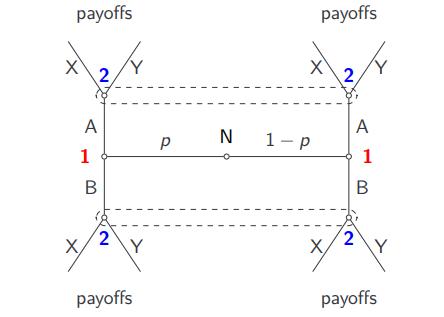
\includegraphics[width=0.5\linewidth]{butt}
    \caption{Representation of the signaling game(butterfly diagram)}
\end{figure}
\Que{Equilibria of signaling games}
\Ans[]{We have 3 kind of equilibria:\begin{itemize}
    \item \textbf{Separating equilibria:} each type of 1 chooses a different action; thus revealing the type to 2
    \item \textbf{Pooling equilibria:} all types of 1 choose the same action; thus, 2 gets no signal about 1's type
    \item \textbf{Intermediate cases:} 1's action does not fully define 1's type, but still provides some information
\end{itemize}}
\Que{Example on butterfly games}
\includepdf[pages=33-52,nup=1x2,landscape=false]{Appendix/Lecture20.pdf}
\Ans[]{Apply the Bayesian rule to the node}
\Que{\textbf{SA1:} consider a dynamic Bayesian game where player 1 moves first and player 2 moves second. Player 1 has three available moves (A,B,C) and only one possible type; player 2 has two available moves (J,K) and two possible types.\begin{itemize}
    \item Draw the game in extensive form (without payoffs)
    \item How many moves specify one strategy of player 1? Why?
    \item How many moves specify one strategy of player 2? Why?
    \item Is SPE enough to characterize the equilibria of the game? Or do you need PBE?
\end{itemize}}
\Que{\textbf{SA2:} Consider a dynamic Bayesian game where player 1 moves first and player 2 moves second. Player 1 has two available moves (C,D) and two possible types $(t_L ,t_R)$ with prior (p,1-p); player 2 has only one type and moves (M,N)
\begin{itemize}
    \item Draw the game in extensive form (without payoffs)
    \item How many moves specify one strategy of player 1? Why?
    \item How many moves specify one strategy of player 2? Why?
    \item Is SPE enough to characterize the equilibria of the game (i.e., to determine wheter a BNE is sequentially rational)? Or do you need PBE?
\end{itemize}}
\Que{\textbf{SA3:} Consider a dynamic Bayesian game where player 1 moves first and player 2 moves second. Player 1 has two available moves (C,D) and two possible types $(t_L ,t_R)$ with prior (p,1-p); player 2 has only one type and moves (M,N)\begin{itemize}
    \item Let $h_D$ be the information set where player 2 moves after observing move D by player 1: what are 2's beliefs values $\mu$ in each node of $h_D$ assuming separating strategy DC for 1?
    \item What are 2's belief values $\mu$ in each node of $h_D$ assuming pooling strategy DD for 1?
    \item What are 2's belief value $\mu$ in each node of $h_D$ assuming pooling strategy CC for 1?
\end{itemize}}